\documentclass[11pt,a4paper,footinclude=true,headinclude=true, oneside]{scrbook}
\usepackage[T1]{fontenc} 
\usepackage{float}
\usepackage{graphicx}
\usepackage{lipsum}
\usepackage{tabu}
\usepackage{booktabs}
\usepackage[linedheaders,parts,pdfspacing]{classicthesis} % ,manychapters
%\usepackage[osf]{libertine}
\usepackage{amsthm}
\bibliographystyle{IEEEtran}
\usepackage{geometry}

\begin{document}

\begin{titlepage}
    \begin{center}
        \vspace*{1cm}
        \begin{figure}[htbp]
            \centerline{
\includegraphics[scale=.5]{ndhu_logo.png}}
        \end{figure}
        {\fontsize{16}{16}\selectfont
            \textbf{Increasing Survivability of UAV Wireless Power Transfer Applied to Wireless Sensor Network Problem in a Mountainous Environment}
        }
        
        \vfill
        \textbf{Student: Vytaras Juraska} \\
        \textbf{Advising Professor: Wei-Che Chien}
        \par\noindent\rule{\textwidth}{0.8pt}
        Master's Thesis\\
        Computer Science and Information Engineering student of\\
        National Dong Hwa University\\
            
    \end{center}
\end{titlepage}

\newgeometry{left=2.5cm,right=4cm,top=2.5cm,bottom=2.5cm,includeheadfoot}

\chapter{Abstract}

Condensed 1 paragraph information about the paper and what it achieves.

\tableofcontents

\chapter{Introduction and Background}

Short introduction to the field of WPT in WSN with UAV: what is it, what each part (WPT, WSN ...) means, what is the main problem that is being solved and what are the most popular ways this problem is ALREADY solved.

\section{State of UAV}

It is important to understand where UAV consumer grade market is right now, how UAVs are performing and what are the main application methods.

Main leading point is, that UAVs mostly are not made for mission planning convenience yet, that their main drawback is inconsistent battery consumption. Really focus on the advertised range and how strongly it can be impacted by environmental differences, such as wind (can drop even bellow 50 \% of maximum advertised survivable operation time).

Mention, that extra weight requires much better performing UAVs, since in this application it is considered to mount WPT device on UAV. Talk about how the range will be impacted even more, if additional attachments were to be mounted on top of the UAV. Mention diminishing returns of making a bigger and stronger UAV to compensate for weight.

Point out the current consumer grade maximum wind limitations for operation.

\section{Concept of Environment Aware UAV}

Describe an ideal situation of how a environment aware UAV would behave and how it could improve not only in this application, but in most outside related mission planning applications.

Do related work analysis of how the paper with wind analysis gets better performance in mission planning than just simple mission planning without that.

\section{Related work to WPT WSN with UAV}

Quick analysis of other papers, focusing on how they define power consumption and environment analysis (2D, 3D, wind resistance, drag force, wind projection analysis...)

\section{Issues with UAV application to WPT WSN}

Mostly focus on more realistic scenarios: Wireless Sensor Network realistically would be more used in environments where it is less easier to have a wired connection between each sensor, that would mean less accessible environments, such as mountainous terrains.

Talk about inconsistencies with winds in various environments, and the importance of environment and wind consideration in this specific field of subject.

\section{Motivation and Contribution}

I have a keen interest from the academic and personal perspective into the field of UAV applications. Since my bachelor's, which was Electronics Engineering, I worked on system design and development of UAV incorporation to precision agriculture. However, the field of WPT WSN with the application of UAVs have peaked my interest, since this field has a lot of depth, which motivated me to learn more about how UAVs work.

As stated in the "Issues with UAV application to WPT WSN" - I noticed, that there is a reoccurring fundamental overlook, when it came to calculating power consumption of UAVs. And as stated in the related work section, many research works heavily rely on a specific power propulsion expression, and state, that UAV speed of movement should be fixed to cruising speed. However I argue, that fixing the speed realistically requires much more consideration, when it comes to real application. The battery usage is already a big constraint in UAV mission planning applications, where depending on the environment, the actual survivability can be even less than half of the expected or advertised survivability duration. Hence finding ways how to improve this aspect can push the field of automated mission planning application of UAVs further.

My contribution comes down to a few improvements for the system. Firstly, I define my environment as a mountainous terrain, which forces me to consider the simulation of UAV actions in a three-dimensional space. Especially when it comes to getting distance between point A and point B, two-dimensional space would yield inaccurate results, since it does not consider the distance difference in the height axis. Secondly, three-dimensional terrain creates a more varied space for winds direction and speeds, since these two properties heavily rely on what kind of terrain does the wind flow through. As mentioned in the section "Concept of Environment Aware UAV", there are a few applicable methods, that I use to simulate the environment and how winds properties would be affected.

Considering power consumption, I found a way to implement wind properties and their affects to UAV speeds - which leads to different UAV power consumption values for propulsion. This part is explained in the "Problem Definition" section. In the environment aware related work, methods were mostly avoiding high wind speed area, but not necessarily measuring power consumption using these properties. Main difference that this makes, is that my implementation not only avoids higher consumption paths, but attempts to utilize tailwind scenarios, where UAV speed naturally increases - minimising power consumption and hence increasing survivability. The prioritisation part comes down to solving TSP problem efficiently, which is an area with various of already efficient solutions and countless amounts of research works surrounding the field.

Since my UAV mission planning application is very specific, I will rely on multiple methods for finding the shortest path, or in my case - smallest cost. This will also be a part of my contribution, is finding a specific, most efficient method of solving smallest cost path planning in the application of UAV WSN WPT problem.

And finally, this field requires clustering methods. Considering my already changed environment from the typically considered one in other works I implement X-Means method for clustering, which prioritises how much is WPT is able to reach and dynamically considers the amount of centroids or WSNs that the environment has to have.

\chapter{Problem Definition}

\section{Cost Calculation}

To effectively understand the survivability of a UAV in the application of recharging WSN with a WPT - I have to consider the cost of battery consumption for each operation that the UAV has to accomplish. Hence we first take this application and consider different areas of power consumption that I will have to define:
\begin{itemize}
  \item UAV power required for propulsion. That includes pushing in the forward movement and pushing downwards when hovering;
  \item WPT power required for charging.
\end{itemize}

\subsection{UAV Power for Propulsion}

Base-line for power consumption cost calculation comes from one of the main sources\cite{zeng2019energy}, which takes apart the popular mathematical expression used for helicopter power consumption calculation and applies it to multi-copter aerial vehicles:

\[ P(V) = P_0  \left( 1 + \frac{3V^2}{U_{tip}^2} \right) 
    + P_i \left( \sqrt{1 + \frac{V^4}{4v_0^4}} - \frac{V^2}{2v_0^4} \right)
    + \frac{1}{2} d_0\rho sAV^3 \]

Where \(P_0\) and \(P_1\) are are constants for blade profile power and induced power, which have their own expressions defined in the same source:

\[ P_0 = \frac{\delta}{8} \rho sA\Omega^3R^3 \]
\[ P_i = (1 + k) \frac{W^{3/2}}{\sqrt{2\rho A}} \]

The variables in these expressions used are as follows:

\begin{itemize}
    \item \(W\) - UAV weight, Newton;
    \item \(\rho\) - air density, \(kg/m^3\);
    \item \(R\) - rotor radius, meter;
    \item \(\Omega\) - angular velocity, radians/second;
    \item \(b\) - number of blades of the UAV;
    \item \(c\) - blade chord length;
    \item \(S_{FP}\) - fuselage equivalent flat plane area, \(m^2\);
    \item \(\delta\) - profile drag coefficient;
    \item \(k\) - incremental correction factor to induced power.
\end{itemize}

Rest of the variables used are calculated using the variables defined above. The calculable variables are:

\begin{itemize}
    \item \(A\) - rotor disc area, \(m^2\): 
        \[ A = \pi R^2\]
    \item \(U_{tip}\) - tip speed of the rotor blade:  
        \[ U_{tip}  = \Omega R\]
    \item \(s\) - rotor solidity, the ratio of the total blade area to the disc area:
        \[ s = \frac{bc}{\pi R} \]
    \item \(d_0\) - fuselage drag ratio:
        \[ d_0 = \frac{S_{FP}}{sA} \]
    \item \(v_0\) - mean rotor induced velocity in hover:
        \[ v_0 = \sqrt{\frac{W}{2\rho A}} \]
\end{itemize}

Hence, having some of the main characteristics of the UAV, the rest of the variables can be found and the main propulsion power can be found. The propulsion expression can be split into three different parts in order to understand what exactly it does, the two of which were already mentioned before: 

\begin{itemize}
    \item Blade profile power, it increases with bigger speed values, it is the power needed to overcome drag force, that is created by the profile of the blades and the drag force, that is generated by the fuselage (main physical body of the UAV);
    \item Induced power, decreases with bigger values of speed, which is the power required for the UAV to maintain enough lift to push against the pull of gravity and overcome the induced drag, that the blades generate.
\end{itemize}

The last part of the main expression is the parasitic power, which is simply the power to overcome drag force, which is generated by the UAV (its body and blades) interacting with the air. It also increases with the bigger values of speed.

The main input for the whole expression is the speed of the UAV. Hence if the UAV is moving, we apply its speed to the equation and we get the output of Watts required to overcome all the forces mentioned above. And if the UAV is hovering in one place, we input speed as zero, which simplifies the whole expression to:

    \[ P_{hover} = P(0) = P_0 + P_i\]


\subsection{Adding Wind Affect to UAV Speed}

The main issue with base-line propulsion power consumption expression, is that there is no consideration for wind, the parasitic power calculation is drag force against no wind air resistance. The change needed to be done, is to modify the expression for power required to overcome drag force against air with a specified wind speed and angle relative to the UAV.

Firstly, an understanding of how wind affects aerial vehicles has to be explained. For example, if UAV speed is 10 m/s and it is flying directly against the wind, which has the speed of 3 m/s, then the actual UAV propulsion speed is going to be 7 m/s. 

 \[V_{pro} = V_{UAV} - V_{wind}\]

\begin{figure}[h]
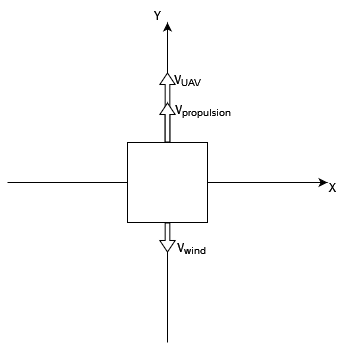
\includegraphics[scale=0.7]{UAV_against_wind.png}
\centering
\end{figure}

When considering drag force of an object being affected by wind, no wind calculation process is the same, the only difference is finding the actual speed, which the object is traveling at. Coming back to the example above, if there would be no wind, we would use the original UAV speed with the drag force expression and get power needed to overcome it, but in a windy environment, according to the angle of the wind impacting the UAV, it changes the UAV propulsion speed, hence applying the changed speed we get different results for the drag force.

This process of simplifying the problem to a singular object speed is fairly common, when considering drag force affected by wind calculations. However, this expression only works, if the wind is directly against the movement of a UAV. Depending on the wind angle, it can either slow down the UAV or increase its speed. If wind is blowing from the back of the UAV, which is called tailwind, it will increase UAVs speed by the amount of winds speed. So now considering, that if wind is in front, it will slow UAV down, and if it is behind - it will speed it up, I define possible angles. Considering negative y axis as 0° angle and negative x axis as 90° angle, I can define:

\[V = V_{UAV} + V_{wind}\ \textrm{when}\ 90 \leq \theta \leq 270\]

\[V = V_{UAV} - V_{wind}\ \textrm{when}\ 0 \leq \theta < 90\ \textrm{and}\ 270 < \theta \leq 360\]

Implementing this we would add or subtract the whole wind speed from or to the UAV, but if the wind is on an angle, then we have to find the exact impact it would have to UAV propulsion speed. The expression can be simply found applying some trigonometry and visualising a possible situation with a free-body diagram:

\begin{figure}[h]
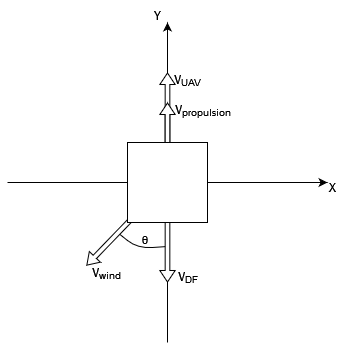
\includegraphics[scale=0.7]{UAV_against_wind_angle.png}
\centering
\end{figure}

In this diagram \(v_{wind}\) is the wind vector, which is on an \(\theta\) angle from the \(V_{DF}\) - which is the actual speed of wind drag force. To solve this, I would apply trigonometric rule of \(cos\theta = \frac{Adjacent}{Hypotenuse}\) to get the value of Adjacent, so in this case Hypotenuse is \(V_{wind}\), where as Adjacent would be \(V_{DF}\), hence when I apply this to the wind impact to UAV speed expression, I get:

\[V_{pro} = V_{UAV} - V_{wind} cos \theta \]

The expression will always be subtracting the two values. This works in my favour, since I need to add the two values at \(90 < \theta < 270\), and \(cos\theta\) at these angles gives a negative value, hence that subtraction changes to addition by itself. And considering the other angles, \(cos\theta\) gives positive values, which results in a subtraction, which is exactly what is needed.

Of course, in reality there is more than one wind affecting UAV speeds, hence realistically the final equation should be:

\[V_{pro} = V_{UAV} - \sum_{i=1}^{n}V_{wind}(i) cos\theta_{wind}(i)\]

Where there would be a numerated \(n\) amount of winds, where each wind would have its individual speed and angle. Summed amount of different speeds would have to be finally subtracted from the main UAV speed to get the final propulsion speed, so if from any specific angle the wind affect would be above the advertised wind speed, UAV would not be able to propel forwards.

However, to not branch the complexity of computation even further, I decided to rely on a singular wind affect, since the rest of the computations do not change from this point on, and the calculations have to compute each of the winds into a singular wind drag force vector, hence the simpler singular wind representation would still be the concluding representation of wind affect.

\subsection{Improved Cost Mathematical Expression}

Having the base-line cost mathematical expression defined, and introduced a way to improve the expression with implementing wind strength and angle consideration I can define the improved cost expression and specify how it will be applied to the whole WPT WSN system:

\[ P_{mov} = P(V = V_{UAV} - V_{wind} cos \theta) = P_0  \left( 1 + \frac{3V^2}{U_{tip}^2} \right) 
    + P_i \left( \sqrt{1 + \frac{V^4}{4v_0^4}} - \frac{V^2}{2v_0^4} \right)
    + \frac{1}{2} d_0\rho sAV^3 \]

Each path that UAV will take is going to be split into smaller segments, where the wind properties are going to be measured at those points. Hence to effectively use this expression, there has to be a wind simulation incorporated into the application part, which will be covered in the "System Design and Functionality" part.

However this expression only give how much power (watts) it would need to achieve that speed to overcome all the previously defined types of forces. To get power consumption we find individual paths, that the UAV would have to traverse and find their distances. And once we know each paths distance, we can divide that distance over UAV propulsion speed to get how much time it will take to reach the end of each path:

\[time = \frac{distance}{speed}\]

And now we can get milliamp-hour, which is a measurement of battery capacity. This would give me how much battery capacity UAV would use to go through that path. Battery capacity expression gives amp-hour, so I also multiply it by 1000 to get milliamphour. I do that, because that seems to be the most common representation of battery capacity, especially when the application requires to deal with small distances. Expression goes as follows: 

\[battery\ capacity\ used = \frac{watthours}{battery\ voltage} * 1000\]

This expression requires the voltage of a battery, that is used by UAV and watt-hours consumed by the UAV. Voltage is received from specifications of batteries and for watt-hours I use a simple equation:

\[watthours = \frac{watts}{(seconds / 3600)}\]

Watts would be the propulsion power. A watt is energy per second, or joule per second, hence to get watt-hour I have to convert the seconds that UAV takes to complete the path to hours and then divide that number from watts. Having all of the necessary expressions defined now I can get exact battery capacity required for the UAV to complete a path at a specific speed impacted by the speed and angle of the wind.

And since there are many paths that the UAV has to take to cover all of the WSNs, the overall battery capacity used would be:

\[total\ battery\ used = \sum_{i=1}^{n} battery\ capacity\ used(path = i) \]

where each possible path would be numerated, there would be total of \(n\) amount of paths, starting from 1. Each path would provide the distance, but the other variables, such as speed and propulsion power would be set individually in previous parts of the calculation.

\section{Wireless Power Transfer Cost Calculation}

This section I will rely on the related work sources for the method of power consumption for WPT. Since I mostly focused on UAV movement computation I will have to apply most of the simplification at this part.

\chapter{System Design and Functionality}

Introduction to what system I created and what it does in a simple form.

\section{Environment Generation and Simulation}

Show methods of how I generate terrain and other methods which take real world terrain and convert it to an iterable list of data points.

Show how I generate sensors.

\section{Grouping Sensors}

Show methods of K-Means and X-Means and how they are used to get centroids, why they are important

\section{UAV motion and path generation}

Show how I get all possible paths that UAV can take, talk about how it manages to navigate in a 3D environment and avoid mountainous terrains.

\section{Measurement implementation}

Show how I get milliamphours.

Show Windninja and how I get simulated results for winds strength and direction in a 3D environment. Show how I apply equations to get angles from the perspective of the UAV and the amount wind speed effects the UAV speed.


\section{Shortest Path}

Show how I get shortest path with ACO and 2-OPT ACO

\section{Plotting}

Show methods of how I visualise data in the end

\chapter{Simulation and Comparison of different Models}

Showing results compared to other methods.

\section{Power Consumtion Improvement Results}
Base model is the non-dynamic power consumption formula which has just drag force. Compare with improved version which uses wind simualted data to get results.

\section{Shortest Path Improvement Results}
Show possible shortest path improvements with 2OPT-ACO and ACO.

\chapter{Discussion}

Condensed description of what the paper achieved, what do my results mean.

\chapter{Conclusion and Future Work}

Talk about Future Work, what could be done to improve the results (since I have 1 topic, mostly focus on that one topic). A* and such.

Talk about how my methods improved the current state of survivability when improving the power consumption calculation methods.

Conclude that improvement is present in any case, since this is more realistic representation of outside environment when considering mission planning with UAVs, and also in this case the models is created with the idea of this specific WPT WSN field.

\bibliography{references}
\chapter{Affidavit}
I, Vytaras Juraska, herewith declare that I have composed the present paper and work by myself and without use of any other than the cited sources and aids. Sentences or parts of sentences quoted literally are marked as such; other references with regard to the statement and scope are indicated by full details of the publications concerned. The paper and work in the same or similar form has not been submitted to any examination body and has not been published. This paper was not yet, even in part, used in another examination or as a course performance.

\begin{figure}[H]
\hspace*{3.5cm}
\centerline{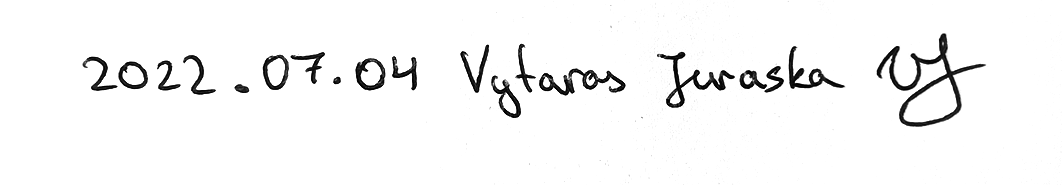
\includegraphics[scale=1]{Signature.png}}
\end{figure}
\end{document}